\section{Standard e metodi per la gestione della Qualità}
  \subsubsection{\glossaryItem{ISO}/\glossaryItem{IEC} 9126 \emph{Software engineering — Product quality}}
  L'obiettivo di questo standard è quello di definire un modello per poter valutar la qualità del software.\\
  Lo standard si divide in quattro parti:
  \begin{itemize}
    \item modello della qualità del software;
    \item metriche per la qualità interna;
    \item metriche per la qualità esterna;
    \item metriche per la qualità in uso.
  \end{itemize}
  \paragraph{Modello della qualità del software}
  Il modello della qualità del software presentato nella prima parte dello standard (\glossaryItem{ISO}/\glossaryItem{IEC} 9126-1), identifica sei caratteristiche generali e varie sottocaratteristiche:
  \begin{enumerate}
    \item \textbf{Funzionalità:}
    \begin{itemize}
        \item \textbf{Adeguatezza}: la capacità del software di offrire un appropriato insieme di funzioni per determinati compiti.
        \item \textbf{Accuratezza}: la capacità del prodotto software di rendere risultati concordati o i precisi effetti aspettati.
        \item \textbf{Interoperabilità}: capacità del prodotto software di operare e interagire con sistemi uno o più sistemi specificati.
        \item \textbf{Sicurezza}: la capacità di proteggere dati e informazioni, impedendo a persone e sistemi non autorizzati di accedervi, e garantendo sempre l'accesso ai dati a persone e sistemi autorizzati.
        \item \textbf{Conformità funzionale}: capacità del prodotto software di aderire a standard, convenzioni e regolamentazioni riguardanti il settore operativo a cui vengono applicate.
    \end{itemize}
    \item \textbf{Affidabilità:}
    \begin{itemize}
      \item \textbf{Maturità}: capacità del prodotto software di evitare il verificarsi di errori, malfunzionamenti o siano prodotto risultati errati.
      \item \textbf{Tolleranza agli errori}: è la capacità del prodotto software di mantenere livelli predeterminati di prestazioni anche in presenza di malfunzionamenti o usi scorretti del prodotto.
      \item \textbf{Recuperabilità}: capacità di ripristinare il livello appropriato di prestazioni e di recupero delle informazioni rilevanti, in seguito a un malfunzionamento.
      A seguito di un errore, il software può risultare non accessibile per un determinato periodo di tempo, questo arco di tempo è valutato proprio dalla caratteristica di recuperabilità.
      \item \textbf{Aderenza}: è la capacità di aderire a standard, regole e convenzioni inerenti all'affidabilità.
    \end{itemize}
    \item \textbf{Usabilità:}
    \begin{itemize}
      \item \textbf{Comprensibilità}: è la capacità del prodotto software di mettere l'utente in grado di comprendere se il software è appropriato, e come esso possa essere usato per scopi e condizioni d'uso particolari
      \item \textbf{Apprendibilità}: è la capacità di ridurre l'impegno richiesto agli utenti per imparare ad usare la sua applicazione.
      \item \textbf{Operabilità}: è la capacità del prodotto software di rendere l'utente in grado di operarlo e controllarlo.
      \item \textbf{Attrattiva}: è la capacità del software di essere piacevole per l'utente.
      \item \textbf{Conformità}: è la capacità del prodotto software di aderire a standard o convenzioni relativi all'usabilità.
    \end{itemize}
    \item \textbf{Efficienza:}
    \begin{itemize}
      \item \textbf{Comportamento rispetto al tempo}: è la capacità di fornire adeguati tempi di risposta, elaborazione e velocità di attraversamento, sotto condizioni determinate.
      \item \textbf{Utilizzo delle risorse}: capacità del prodotto software di usare un adeguato quntitativo e tipo di risorse quando il software esegue le sue funzioni in determinate condizioni.
      \item \textbf{Conformità}: è la capacità di aderire a standard e specifiche sull'efficienza.
    \end{itemize}
    \item \textbf{Manutenibilità:}
    \begin{itemize}
      \item \textbf{Analizzabilità}: è la del prodotto software di essere facilmente controllato per la ricerca di errori, o di facilitare l'identificazione delle parti che devono essere modificate.
      \item \textbf{Modificabilità}: capacità del prodotto software di rendere possibili eventuali implementazioni di modifiche.
      \item \textbf{Stabilità}: la capacità del prodotto software di evitare effetti indesiderati dovuti alle modifiche del software stesso.
      \item \textbf{Testabilità}: è la capacità del prodotto software di poter validare le modifiche ad esso apportate
      \item \textbf{Conformità di manutenibilità}: è la capacità di aderire a standard e specifiche riguardanti la manutenibilità.
    \end{itemize}
    \item \textbf{Portabilità:}
    \begin{itemize}
      \item \textbf{Adattabilità}: la capacità del software di essere adattato per differenti ambienti operativi senza dover applicare modifiche diverse da quelle fornite per il software considerato.
      \item \textbf{Installabilità}: la capacità del software di essere installato in uno specificato ambiente.
      \item \textbf{Sostituibilità}: è la capacità di essere utilizzato al posto di un altro software per svolgere gli stessi compiti nello stesso ambiente.
      \item \textbf{Conformità}: la capacità del prodotto software di aderire a standard e convenzioni relative alla portabilità.
    \end{itemize}
  \end{enumerate}

  \paragraph{Metriche per la qualità interna}
    Le metriche per la qualità interna o mentriche interne, descritte nel \emph{technical report} \glossaryItem{ISO}/\glossaryItem{IEC} 9126-3,
    sono delle metriche che si applicano al software non eseguibile durante le fasi di progettazione e codifica.
    Le metriche interne permettono di individuare eventuali problemi che potrebbero influire sulla qualità finale del prodotto prima che sia realizzato il software eseguibile
    Le misure effettuate permettono di prevedere il livello di qualità esterna ed in uso del prodotto finale,
    poiché gli attributi interni influiscono su quelli esterni e quelli in uso.

  \paragraph{Metriche per la qualità esterna}
    Le metriche per la qualità esterna o metriche esterne, descritte nel \emph{technical report} \glossaryItem{ISO}/\glossaryItem{IEC} 9126-2,
    sono delle metriche adatte alla misurazione dei comportamenti del software sulla base di misure ottenute da test, oparando e osservando il software eseguibile o sistema stesso.

  \paragraph{Metriche per la qualità in uso}
    Le metriche per la qualità in uso misurano il grado con cui il prodotto software permette agli utenti di svolgere le proprie attività con efficacia, produttività, sicurezza e soddisfazione nel contesto operativo previsto.
    Questa valutazione è quindi fatta in specifici scenari d'uso.\\
    La qualità deriva anche dall'effetto combinato di più caratteristiche interne ed esterne di qualità.
    Il \emph{technical report} \glossaryItem{ISO}/\glossaryItem{IEC} 9126-4 fornisce alcune metriche per la misurazione della qualità in uso.

  \begin{figure}
    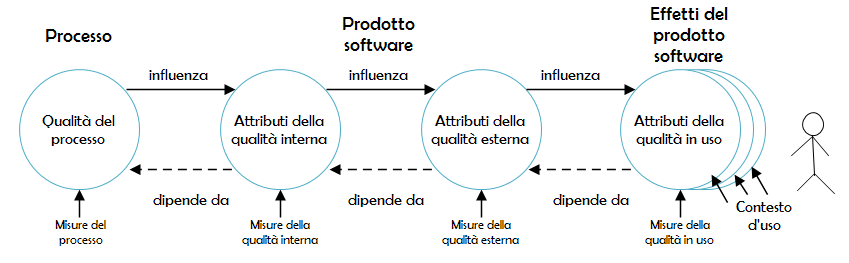
\includegraphics[width=1\textwidth]{res/sections/img/qdps.png}
    \caption{Ciclo di qualità del software}
    \centering
    \label{}
  \end{figure}


  \subsubsection{\glossaryItem{ISO}/\glossaryItem{IEC} 15504 \emph{Information technology – Process assessment}}

  \glossaryItem{ISO}/\glossaryItem{IEC} 15504, anche conosciuta come SPICE (Software Process improvement and Capability Determination),
  è un insieme di nove documenti di standard tecnici relativi ai processi di sviluppo del software e relative funzioni di business e, in particolare, alla loro valutazione.

  \paragraph{Modello di riferimento}
  \glossaryItem{ISO}/\glossaryItem{IEC} 15504 presenta un modello di riferimento che definisce una dimensione del processo e una della capacità.\\
  La dimensione del processo definisce processi divisi in cinque categorie di processo:
  \begin{itemize}
    \item \emph{customer/suplier};
    \item \emph{engineering};
    \item \emph{supporting};
    \item \emph{management};
    \item \emph{organization}.
  \end{itemize}
  La dimensione della capacità definisce una scala di maturità a cinque livelli (più il livello base, detto livello 0) così definiti:
  \begin{itemize}
    \item \emph{Level 5: Optimizing process};
    \item \emph{Level 4: Predictable process};
    \item \emph{Level 3: Established process};
    \item \emph{Level 2: Managed process};
    \item \emph{Level 1: Performed process};
    \item \emph{Level 0: Incomplete process}.
  \end{itemize}
  La capacità dei processi è misurata tramite gli attributi definiti a livello internazionale e che sono:
  \begin{itemize}
    \item \emph{1.1 Process performance};
    \item \emph{2.1 Performance management};
    \item \emph{2.2 Work product management};
    \item \emph{3.1 Process definition};
    \item \emph{3.2 Process deployment};
    \item \emph{4.1 Process measurement};
    \item \emph{4.2 Process control};
    \item \emph{5.1 Process innovation};
    \item \emph{5.2 Process optimization}.
  \end{itemize}
  Ogni attributo del processo consiste di una o più pratiche generiche, le quali sono ulteriormente elaborate in "Indicatori della pratica" che aiutano nella fase di valutazione delle prestazioni.
  \\Ciascun attributo del processo è valutato seconod una scala di quattro valori (N-P-L-F):
  \begin{itemize}
    \item \emph{Not achieved} (0 - 15\%);
    \item \emph{Partially achieved} (>15\% - 50\%);
    \item \emph{Largely achieved} (>50\% - 85\%);
    \item \emph{Fully achieved} (>85\% - 100\%).
  \end{itemize}
  La valutazione si basa su prove raccolte fronte di ciascun indicatore di processo durante la fase di valutazione.

  \paragraph{Valutazione}
  \glossaryItem{ISO}/\glossaryItem{IEC} 15504 fornisce una guida per effettuare una verifica dei processi:
  \begin{itemize}
    \item il processo di valutazione (\emph{the assessment process});
    \item il modello di valutazione (\emph{the model for the assessment});
    \item tutti strumenti per effettuare la valutazione (\emph{any tools used in the assessment}).
  \end{itemize}
  \paragraph{Processo di valutazione}
  Eseguire la valutazione dei processi è oggetto della parte 2 e 3 del \glossaryItem{ISO}/\glossaryItem{IEC} 15504.\\
  Il processo di valutazione può essere generalizzato nei seguenti passi:
  \begin{itemize}
    \item inizio dell'assessment;
    \item selezione del valutatore e del team di valutazione;
    \item pianificazione dell'assessment, inclusa la definizione dei processi e dell'organizzazione da valutare;
    \item riunione preliminare;
    \item raccolta dei dati;
    \item validazione dei dati raccolti;
    \item valutazione del processo;
    \item rapporto sul risultato della valutazione.
  \end{itemize}

  \subsubsection{Ciclo di Deming o ciclo di Shewhart}
  Il ciclo di Deming (o ciclo di Shewhard) detto anche PDCA (o PDSA) si compone di 4 fasi:
  \begin{itemize}
    \item \textbf{P - Plan}: questa fase stabilisce gli obiettivi e processi necessari all'ottenimento dei risultati coerenti ai risultati attesi;
    lo stabilire le aspettative di risultati, la completezza e accuratezza delle specifice scelte sono parte del miglioramento mirato.
    Iniziare su piccola scala, quando possibile, per poter verificare possibili effetti.
    \item \textbf{D - Do}: Implementazione della fase \emph{Plan}, esecuzione del processo, creazione del prodotto.
    Raccogliere i dati per la creazione di grafici e analisi da destinare alla fase di "Check" e "Act".
    \item \textbf{C - Check(or S - Study)}: Controllo e studio dei risultati raccolti nella fase \emph{Do}. Confrontare i risultati con quelli attesi, stabiliti nella fase \emph{Plan}.
    \item \textbf{A - Act}: Azione per rendere definitivo e/o migliorare il processo. L'informazione ottenuta nella fase \emph{Check} è utile per poter individuare i possibili punti di un processo dove apportare modifiche.
  \end{itemize}
